% Autor: Leonhard Segger, Alexander Neuwirth
% Datum: 2017-10-30
\documentclass[
	% Papierformat
	a4paper,
	% Schriftgröße (beliebige Größen mit „fontsize=Xpt“)
	12pt,
	% Schreibt die Papiergröße korrekt ins Ausgabedokument
	pagesize,
	% Sprache für z.B. Babel
	ngerman
]{scrartcl}

% Achtung: Die Reihenfolge der Pakete kann (leider) wichtig sein!
% Insbesondere sollten (so wie hier) babel, fontenc und inputenc (in dieser
% Reihenfolge) als Erstes und hyperref und cleveref (Reihenfolge auch hier
% beachten) als Letztes geladen werden!

\usepackage{tikz}
\usetikzlibrary{calc,patterns,angles,quotes} % loads some tikz extensions\usepackage{tikz}
\usetikzlibrary{babel}

% Silbentrennung etc.; Sprache wird durch Option bei \documentclass festgelegt
\usepackage{babel}
% Verwendung der Zeichentabelle T1 (Sonderzeichen etc.)
\usepackage[T1]{fontenc}
% Legt die Zeichenkodierung der Eingabedatei fest, z.B. UTF-8
\usepackage[utf8]{inputenc}
% Schriftart
\usepackage{lmodern}
% Zusätzliche Sonderzeichen
\usepackage{textcomp}

% Mathepaket (intlimits: Grenzen über/unter Integralzeichen)
\usepackage[intlimits]{amsmath}
% Ermöglicht die Nutzung von \SI{Zahl}{Einheit} u.a.
\usepackage{siunitx}
% Zum flexiblen Einbinden von Grafiken (\includegraphics)
\usepackage{graphicx}
% Abbildungen im Fließtext
\usepackage{wrapfig}
% Abbildungen nebeneinander (subfigure, subtable)
\usepackage{subcaption}
% Funktionen für Anführungszeichen
\usepackage{csquotes}
\MakeOuterQuote{"}
% Zitieren, Bibliografie
\usepackage[sorting=none]{biblatex}


% Zur Darstellung von Webadressen
\usepackage{url}
%chemische Formeln
\usepackage[version=4]{mhchem}
% siunitx: Deutsche Ausgabe, Messfehler getrennt mit ± ausgeben
\usepackage{floatrow}
\floatsetup[table]{capposition=top}
\usepackage{float}
% Verlinkt Textstellen im PDF-Dokument
\usepackage[unicode]{hyperref}
% "Schlaue" Referenzen (nach hyperref laden!)
\usepackage{cleveref}
\sisetup{
	locale=DE,
	separate-uncertainty
}
\bibliography{BA-C-04_MP1_21-01-2019_References}

\begin{document}

	\begin{titlepage}
		\centering
		{\scshape\LARGE Versuchsbericht zu \par}
		\vspace{1cm}
		{\scshape\huge MP1 - Eigenschaften der Solarzelle \par} %TODO Iwie ist der Titel nur 50% -> tja, ist aber so
		\vspace{2.5cm}
		{\LARGE Gruppe BA-C-04 \par}
		\vspace{0.5cm}

		{\large Alexander Neuwirth (E-Mail: a\_neuw01@wwu.de) \par}
		{\large Leonhard Segger (E-Mail: l\_segg03@uni-muenster.de) \par}
		\vfill

		durchgeführt am 21.01.2019\par
		betreut von\par
		{\large Finn Kutschmann}

		\vfill

		{\large \today\par}
	\end{titlepage}
	\tableofcontents
	\newpage


	\section{Kurzfassung}
	% Hypothese	und deren Ergebnis, wenn Hypothese ist, dass nur Theorie erfüllt, sagen: Erwartung: Theorie aus einführung (mit reflink) erfüllt
	% Ergebnisse, auch Zahlen, mindestens wenn's halbwegs Sinn ergibt
	% Was wurde gemacht
	% manche leute wollen Passiv oder "man", manche nicht
	Aufgrund von Energiewende bzw. CO2-Ausstieg sind Solarzellen auf der Prioritätenliste der Forschung weit nach oben gerückt.
	In diesem Versuch sollen Halbleiter als Grundlage der Solarzelle untersucht werden und zusätzlich die Eigenschaften zweier Solarzellen untersucht werden.

	Es können die Ladungsträgerkonzentrationen verschiedener Halbleiterproben mithilfe der Vierspitzenmethode bestimmt werden.
	Dabei kann die Angabe auf dem beiliegenden Zettel bezüglich der Probe, die als intrinsisch markiert ist, als korrekt gezeigt werden.
	Außerdem wird ein Höhenprofil der Ladungsträgerkonzentration in einer Probe mit vollständiger Phosphordotierung und beidseitiger Ga-Diffusion mit begrenzter Eindringtiefe angefertigt.
	Hierbei kann die Angabe der Diffusionstiefe von etwa \SI{70}{\micro \meter} bestätigt werden.

	Dann werden zwei verschiedene Solarzellen auf ihre Eigenschaften untersucht.
	Unter anderem wird hier der Maximum Power Point (MPP, Punkt der maximalen Leistung) und der Füllfaktor bei verschiedenen Temperaturen und Bestrahlungen bestimmt.
	Ein Vergleich zwischen den Solarzellen ist jedoch nicht möglich.

  \section{Theorie}
	% wdh. Texte
	% wdh. Besprechung


	%TODO siehe Methoden gegen dopplung

	\subsection{Halbleiter}
	%TODO dotierkram allgemein
	Um die Solarzelle verstehen zu könne, muss man zunächst dotierte Halbleiter und die Diode verstehen.
	Halbleiter zeichnen sich dadurch aus, dass sie im Gegensatz zu Leitern eine Bandlücke zwischen Valenz- und Leitungsband besitzen, welche gleichzeitig im Vergleich zu Isolatoren sehr gering ist.
	Im folgenden werden elementare Halbleiter der vierten Hauptgruppe betrachtet, aber die Erklärungen lassen sich auch auf andere Halbleiter ausweiten.
	Andere Halbleiter sind beispielsweise aus Elementen der dritten und fünften Hauptgruppe zusammengesetzt.
	Das prominenteste Beispiel hierfür ist Galliumarsenid.

	Bei Raumtemperatur befinden sich in Halbleitern nur wenige Ladungsträger im Leitungsband, weshalb der spezifische Widerstand groß ist.
	Wenn nun Elemente aus der fünften Hauptgruppe (Donatoren) in das Gitter eingebracht werden, nennt man das n-Dotierung, da die eingebrachten Elemente ein Elektron zu viel in der äußeren Schale haben, um sich optimal in das Gitter einfügen zu können.
	Das führt dazu, dass dieses Elektron nicht fest am Atomrumpf sitzt, sondern durch thermische Anregung leicht ins Leitungsband befördert werden kann und somit der spezifische Widerstand sinkt bzw. die Leitfähigkeit steigt. %TODO glaube diese Erkenntnis stammt aus PkM
	Analog kann mit Elementen aus der dritten Hauptgruppe (Akzeptoren) dotiert werden.
	Dies führt zu fehlenden Elektronen im Gitter, sodass mit einer geringen thermischen Anregung ein Elektron von einem benachbarten Atom in die Fehlstelle springen kann.
	Jetzt liegt die Fehlstelle an dem anderen Atom, zu dem wiederum ein anderes Elektron springen kann.
	Das Loch ist also beweglich und erlaubt einen Ladungstransport, weshalb auch hier der Widerstand sinkt.

	\subsubsection{pn-Übergang}
	Wenn man einen p-dotierten Halbleiter in direkten Kontakt mit einem n-dotierten bringt oder einfach einen Halbleiter an zwei Seiten unterschiedlich dotiert, nennt man dies einen pn-Übergang.

	Aus energetischen Gründen wandern dann Elektronen und Löcher aufeinander zu und rekombinieren in der Übergangszone.
	Da hierbei jedoch im n-dotierten Halbleiter Atome mit einem Elektron weniger zurückgelassen werden, als sie Protonen im Kern haben, beginnt sich auf dieser Seite des Halbleiters eine positive Gesamtladung zu sammeln.
	Gleichzeitig erhalten die Atome im p-dotierten Halbleiter ein Elektron mehr, als sie Protonen im Kern haben, sodass sich hier eine negative Gesamtladung sammelt.

	Das elektrische Feld, das durch die Ladungsdifferenz entsteht wirkt energetisch der Rekombination entgegen, sodass sich ein Gleichgewicht mit einer Raumladungszone zwischen den Halbleitern einstellt.
	Diese Raumladungszone sorgt für die vielfältigen Eigenschaften des pn-Übergangs, der auch Diode genannt wird:
	Wird eine Spannung so angelegt, dass der Pluspol am p-dotierten Halbleiter liegt, baut diese die Raumladungszone ab und es kommt zu einem exponentiellen Anstieg der Stromstärke.
	Wird die Spannung andersherum angelegt, wird die Raumladungszone verbreitert und die Diode sperrt, sodass der Stromfluss gering (Null) ist.

	Die Diode wird charakterisiert durch die Diodenkennlinie, die die Abhängigkeit vom Stromfluss zur angelegten Spannung angibt und idealerweise der folgenden Gleichung gehorcht:
	\begin{equation}
		\label{eq_diode_ideal}
		I = I_0 \left[ \exp \left( \frac{eU}{n k_B T} \right) -1 \right] %TODO prüfen, ob das schön ist, weil kann ich nicht
	\end{equation}

	In realen Dioden (besonders Solarzellen) treten jedoch ohmsche Verluste auf, was die Beschreibung durch eine ideale Diode, die mit einem Widerstand in Reihe ( $ R_\text{sh} $ ) und einem anderen parallel ( $ R_\text{s} $ ) geschaltet wurde, erforderlich macht.
	Dadurch wird \cref{eq_diode_ideal} folgendermaßen modifiziert:

	\begin{equation}
		\label{eq_diode_real}
		I = I_0 \left[ \exp \left( \frac{e (U-I R_\text{s})}{n k_B T} \right) -1 \right] + \frac{U-I R_\text{s}}{R_\text{sh}}%TODO prüfen, ob das schön ist, weil kann ich nicht
	\end{equation}

	\subsection{Solarzelle}

	In der Solarzelle wird ein pn-Übergang verwendet, der so offengelegt wird, dass das Licht auf ihn fallen kann.
	Wenn dies der Fall ist, geben die Photonen den Elektronen im Halbleiter die nötige Energie, um die Elektronen aus dem Gitter zu lösen, sodass ein Elektron-Loch-Paar entsteht.
	Wenn dieses Paar in die Raumladungszone diffundiert, bevor es rekombiniert, wird es dort durch das elektrische Feld getrennt.
	Wenn die beiden Enden des pn-Übergangs jetzt über einen Widerstand (oder einen anderen Verbraucher) leitend verbunden werden, können die von den Löchern getrennten Elektronen über den Widerstand rekombinieren, an dem dementsprechend ein Strom gemessen werden kann.
	Dieser Photostrom fließt in Sperrrichtung und modifiziert die ideale Diodengleichung \label{eq_diode_real} wie folgt:

	\begin{equation}
			\label{eq_photostrom}
			I = I_0 \left[\exp{\left(\frac{eU}{n k_B T}\right)}-1\right]-I_\text{ph}
	\end{equation}

	In \cref{fig_photodiode_kennlinie} ist dargestellt, wie dieser Vorang im Banschema aussieht und wie die durch den Photostrom modifizierte Diodenkennlinie aussieht.
	Wenn ein Photodetektor gebaut werden sollte, der einen linearen Zusammenhang zwischen Stromfluss und einfallenden Photonen herstellen soll, würde eine Spannung angelegt werden und der dritte Quadrant wäre relevant.
	Da jedoch eine möglichst hohe Leistung erzielt werden soll, wird bei der Solarzelle der vierte Quadrant verwendet.
	Die Spannung entsteht hier aufgrund des Stromflusses und muss nicht extern angelegt werden.
	Wenn der Widerstand des Widerstands, über den die Enden des Halbleiters verbunden sind, verschwindet stellt sich der sog. Kurzschlussstrom $ I_\text{sc} = - I_\text{ph}$ ein.
	Wenn andersherum keine Verbindung besteht (unendlich großer Widerstand) stellt sich die Leerlaufspannung $ U_\text{oc}$ ein.
	Für die Anwendung soll im Allgemeinen die Leistung maximiert werden, weshalb der sog. Maximum Power Point (MPP) gesucht wird, welcher sich bei der Leistung
	\begin{equation}
			\label{eq_mpp}
			P_\text{max} = I_\text{sc} \cdot U_\text{oc} \cdot FF
	\end{equation}
	ergibt.
	$FF$ ist dabei der Füllfaktor, der von der Bauart der Solarzelle abhängt.
	%TODO der Rest der Formeln für FF und eta ist unten, deswegen lass ich das jetzt so.
	Abschließend ist der Begriff der Luftmasse zu erklären.
	Ein AM-Filter (Air Mass) simuliert die Bedingungen für Solarzellen auf der Erdoberfläche, indem er aus dem Spektrum einer Lampe die Wellenlängen herausfiltert, die auch die Atmosphäre aus dem Sonnenspektrum herausfiltert.
	Eine Luftmasse von eins entspricht dabei dem Weg durch die Atmosphäre, den das Licht bei einem senkrechten Einfall auf die Erdoberfläche zurücklegt.


	\begin{figure}[H]
			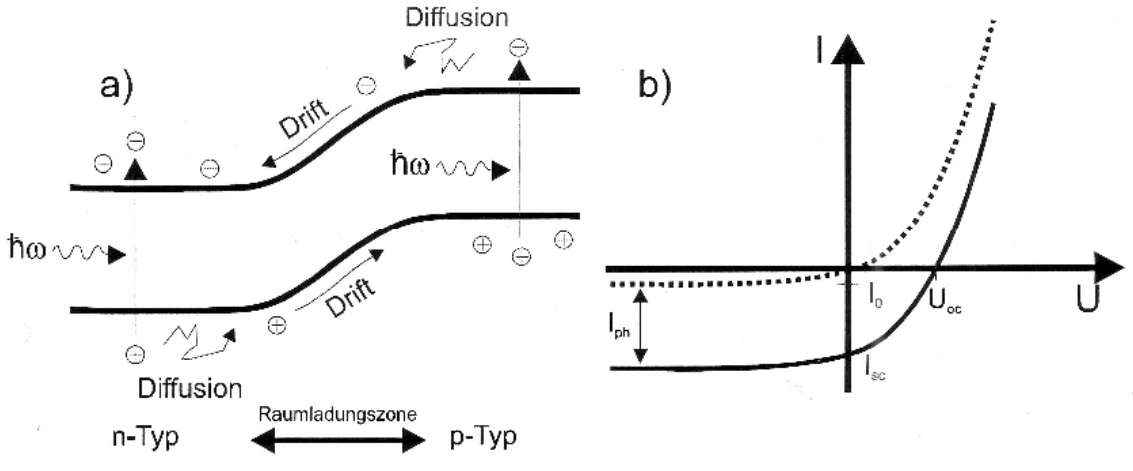
\includegraphics[width= 0.8 \linewidth]{img/photodiode} %TODO prüfen, ob die caption schön ist, weil kann ich nicht.
			\caption{
			a) pn-Übergang unter Beleuchtung: Die photogenerierten Minoritätsladungsträger diffundieren zunächst zur Raumladungszone und werden dort durch das elektrische Feld getrennt
			b) Strom-Spannungs-Charakteristik einer Solarzelle. Die Kennlinie ergibt sich aus der Summe von Diodenstrom $ I $ und Photostrom $ I_\text{ph} $ (negatives Vorzeichen!).
			\cite{anleitung}
			}
			\label{fig_photodiode_kennlinie}
	\end{figure}


	%TODO dein Kram:
	\iffalse
	-allgemeine Formel
	-sehr dünne schichten Korrekturfaktor 1
	-hier: ...kp
	\fi

	\section{Methoden}
	% Bilder von der Website klauen
	% einer will Präsens
	\subsection{Solarzellen}
	Da der vorliegende Versuchsaufbau fehlerhaft war und es nicht möglich war die Messungen zur Solarzelle durchzuführen, wird hier nur das grundsätzliche Vorgehen beschrieben.

	Es sollen für eine Tandemsolarzelle und eine Solarzelle aus polykristallinem Silizium I-U-Kennlinien aufgenommen werden.
	Dies wird ohne Beleuchtung der Solarzellen, bei vollständigem Sonnenspektrum und bei einem AM-gefilterten Sonnenspektrum bei verschiedenen Temperaturen durchgeführt.
	Dazu wird an die Zellen eine Spannung angelegt, die schrittweise erhöht wird.
	Bei Beleuchtung könnte auch der Lastwiderstand variiert werden, um die I-U-Kennlinie aufzunehmen.
	Dies würde jedoch das Messen negativer Spannungen unmöglich machen, die so in die Fit-Funktion mit einbezogen werden können.

	\subsection{Vierspitzenmethode}
	Die Vierspitzenmethode ermöglicht die Messung des Widerstands zwischen den Spitzen in einer dünnen Probe.
	Dazu werden vier Spitzen, dies sich unter gleichem Abstand in einer Linie befinden, auf die Probenoberfläche gedrückt.
	Über die äußeren beiden lässt das Gerät dann einen bekannten Strom fließen und misst die Potenzialdifferenz zwischen den mittleren beiden.
	Die Vierspitzenmethode basiert auf dem Prinzip der Vierleitermessung nach Thomson und Kelvin, die es erlaubt den untersuchten Widerstand unabhängig vom Anschlusswiderstand (hier dem Übergangswiderstand Spitze zu Probe) zu bestimmen.

	\subsection{Dotierstoffe}
	Es wird ein Gerät verwendet, dass die Vierspitzenmethode verwendet, um den spezifischen Widerstand der zu untersuchenden Halbleiter zu bestimmen.
	Dazu werden jeweils zehn Messungen des Widerstands durchgeführt und dann fünf mal mit einem digitalen Mikrometer die Dicke der Probe gemessen, um wissen zu können, ob ein Korrekturfaktor bei der Bestimmung des Widerstands nötig ist.
	Untersucht werden unterschiedlich dotierte Silizium- und Germaniumproben.
	Den Proben liegt ein Zettel bei, der angibt, ob sie p- oder n-dotiert oder intrinsisch sind.

	Zusätzlich wird eine Silizium-Scheibe untersucht, die vollständig mit Phosphor dotiert und dann von beiden Seiten mit Gallium dotiert wurde.
	Dadurch ergibt sich eine tiefenabhängige Dotierung, die untersucht werden soll, indem schrittweise Schichten abgetragen werden und jeweils wie oben die Dicke und der Widerstand gemessen.

	\section{Ergebnisse und Diskussion}

	\subsection{Dotierstoffe}
	\subsubsection{Unsicherheiten}
	Folgende Unsicherheiten werden angenommen:
	\begin{description}
		\item[Mikrometerschraube:]  Digitalanzeige, Rechteckverteilung, da sich jedoch nach einigen Messungen die kalibrierte Nullposition geändert hat, wird die Unsicherheit größer mit $u(x)=\SI{1.7}{\mu m}$ abgeschätzt.
		\item[Vierspitzenmessgeräts:] Digitalanzeige, Rechteckverteilung
	\end{description}
	\subsubsection{Beobachtung und Datenanalyse}

	%\subsubsection*{Dotierungskonzentrationen} %TODO Dotierungs oder Dotierung - konz. -> eigentlich ja Ladungsträgerkonzentrationen
	Mit der Vierspitzenmethode wurde der Widerstand $R=U/I$ gemessen.
	Daraus lässt sich dann mittels der Scheibendicke $d$ der spezifische Widerstand bestimmen.
	\begin{equation}
			\rho = \frac{R d \pi}{\ln 2} \cdot F(d/s)
			\label{eq_spez_wd}
	\end{equation}
	\begin{equation}
			u(\rho) = \rho\cdot\sqrt{(u(R)/R)^2 + (u(d)/d)^2}
	\end{equation}
	Für dünne Scheiben ($d/s<0.5$, $s=\SI{1.59}{mm}$ Messspitzenabstand) ist der Korrekturfaktor gleich 1.
	Für dicke Scheiben erhält man einen Korrekturfaktor F(d/s) ungleich 1 gemäß der DIN-Norm\cite{DIN50431}.
	Dieser beträgt für Probe 4 $F=0.84$ und für Probe 5 $F=0.83$.

	In \cref{tb_spez_wd} befinden sich die gemittelten Messergebnisse.

	\begin{table}[H]
		\centering
		\begin{tabular}{c | c | c | c | c | c  }
			 Nr.& Mat. & dot. & Widerstand $R/\si{\ohm}$& Scheibendicke $d/\si{mm}$ & spez. Widerstand $\rho/\si{\ohm cm}$ \\ \hline %TODO fix overflow
			 1& Si& p& \SI{50+-4}{}&\SI{0.4486+-0.0009}{}& \SI{10.1+-0.7}{} \\
			 2& Si& n&\SI{8.52+-0.21}{}&\SI{0.4532+-0.0009}{}&\SI{1.75+-0.04}{} \\
			 3& Si& n&\SI{0.0713+-0.0018}{}&\SI{0.0677+-0.001}{}&\SI{0.0219+-0.0005}{} \\
			 4& Si& p&\SI{0.00192+-0.00004}{}&\SI{1.999+-0.005}{}&\SI{0.00146+-0.00003}{} \\ %TODO eher als e/10 potenz?
			 5& Ge& i&\SI{25+-5}{}&\SI{2.1070+-0.0013}{}&\SI{19.92+-3.32}{}  \\ %TODO i-dot fine?
			 6& Si& n&\SI{0.084+-0.007}{}&\SI{0.6826+-0.0009}{}&\SI{0.0260+-0.0022}{} \\
		\end{tabular}
		\caption{
		%TODO caption hier
		Gemessene Widerstände und Scheibendicken verschiedener Proben.
		Diese sind p/n-dotiert oder intrinsisch.
		Aus \cref{eq_spez_wd} folgt der spezifische Widerstand.
		}
		\label{tb_spez_wd}
	\end{table}

	Die Ladungsträgerkonzentrationen lassen sich mittels
	\begin{equation}
			\frac{1}{\rho}=en\mu_n + ep\mu_p
	\end{equation}
	bestimmen.
	Für kristallines Silizium bei $T=\SI{300}{K}$ gilt $c=n\cdot p=\SI{2.1e19}{cm^{-6}}$ und die Beweglichkeiten $\mu$ sind nach \cref{tb_beweg} gegeben.


	\begin{table}[H]
		\centering
		\begin{tabular}{c | c | c  }
			 &$\mu_n$ in \si{cm^2/V/s}&$\mu_p$ in \si{cm^2/V/s}\\ \hline
			 Si&1350&480 \\
			 Ge&3900&1900 \\
		\end{tabular}
		\caption{
		Beweglichkeitsdaten für Silizium und Germanium bei $T=\SI{300}{K}$. Entnommen aus \cite{anleitung}. %TODO Ich war mal so frei, dass hier zu addieren, lol du hast den Punkt am Ende vergessen
		}
		\label{tb_beweg}
	\end{table}

	Es ergibt sich:
	\begin{equation}
		\label{eq_n}
			n =  \pm\sqrt{\left(\frac{1}{2e\mu_n\rho}\right)^2-c\mu_p/\mu_n}+\frac{1}{2e\mu_n \rho} %TODO u(n)?
	\end{equation}
	bzw.
	\begin{equation}
			\label{eq_p}
			p =\frac{c}{n}=  \mp\sqrt{\left(\frac{1}{2e\mu_p\rho}\right)^2-c\mu_n/\mu_p}+\frac{1}{2e\mu_p \rho} %TODO u(p)?
	\end{equation}
	Aus der Anleitung sind typische Größenordnungen für n/p-Dotierungkonzentrationen gegeben, woraus folgt, dass für n-dotierte das Vorzeichen vor der Wurzel in \cref{eq_n} positiv und für p-dotierte negative ist.

	Für die intrinsische Ge-Probe gilt $n_i=n=p$.  %SRC https://www.tf.uni-kiel.de/matwis/amat/mw_for_et/kap_9/backbone/r9_1_1.html
	Also:
	\begin{equation}
		\label{eq_ni}
			n_i = \frac{1}{ \rho e (\mu_n+\mu_p)}
	\end{equation}
	\begin{table}[H]
		\centering
		\begin{tabular}{ c | c | c | c | c | c }
			 Nr.&Mat.& dot.& n in \si{cm^{-3}}&p in \si{cm^{-3}}& DIN in \si{cm^{-3}}\\ \hline

			 1&Si&p&\SI{1.63+-0.12e+04}{}&\SI{1.29+-0.09e+15}{}&$p=\SI{1.33e+14}{}$\\
			  2 &Si&n& \SI{2.64+-0.07e+15}{}&\SI{7.95+-0.20e+03}{}&$n=\SI{2.77e+15}{}$ \\
			  3&Si&n& \SI{2.11+-0.05e+17}{}& \SI{99.3+-2.5}{}& $n=\SI{1.09e18}{}$\\
			 4 &Si&p&\SI{2.36+-0.05}{}&\SI{8.90+-0.20e+18}{}& $p=\SI{7.68e+19}{}$\\
			 5 & Ge&i&\SI{ 5.5+-1.0e+13}{}&\SI{5.5+-1.0e+13}{}& \\
			 6 & Si&n&\SI{1.78+-0.15e+17}{}&\SI{118+-10}{}&$n=\SI{7.94e17}{}$\\
		\end{tabular}
		\caption{
		Aus den spezifischen Widerständen $\rho$ folgende Dotierungskonzentrationen.
		Diese wurden einmal mit \crefrange{eq_n}{eq_ni} und einmal mittels einer Tabelle aus der DIN-Norm\cite{DIN50431} bestimmt.
		}
		\label{tb_dot_konz}
	\end{table}

	In \cref{fig_polier_wdst} ist die Widerstandsmessung der phosphordotierten Si-Scheibe mit Ga-Diffusion gegen den Schichtenabtrag abgebildet.
	Der Widerstand erreicht ein Maximum bei \SI{65+-2}{\mu m}.

	\begin{figure}[H]
			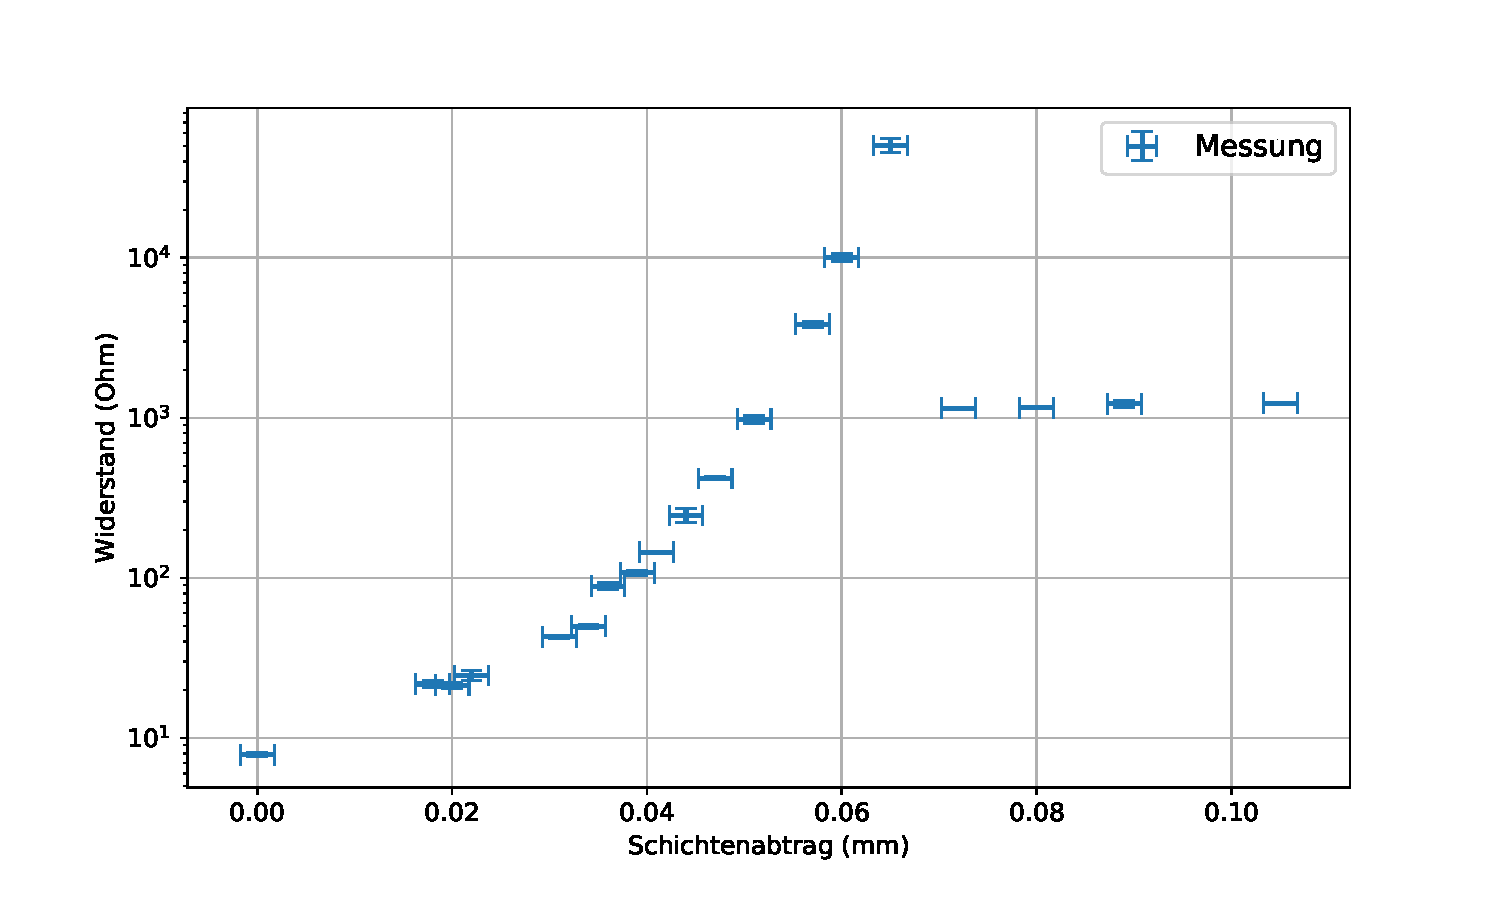
\includegraphics[width=.9\linewidth]{img/polier_wdst.pdf}
			\caption{
			Der Widerstand $R$ wird durch die Vierspitzenmethode gemessen und die Oberfläche wird schichtweise abgetragen.
			}
			\label{fig_polier_wdst}
	\end{figure}

	Der spezifische Widerstand ergibt sich aus
	\begin{equation}
		\frac{1}{\rho} = - \frac{\ln 2}{\pi} \frac{d}{dx}R^{-1},
	\end{equation}
	bzw. numerisch
	\begin{equation}
		\frac{1}{\rho_i} = - \frac{\ln 2 }{\pi} \frac{R^{-1}_{i+1}-R^{-1}_{i}}{x_{i+1}-x_i}.
	\end{equation}
	Man erhält durch Einsetzten in \cref{eq_p} die Löcherkonzentration.
	Diese ist in Abhängingkeit vom Schichtenabtrag in \cref{fig_polier_konz} dargestellt.

	\begin{figure}[H]
			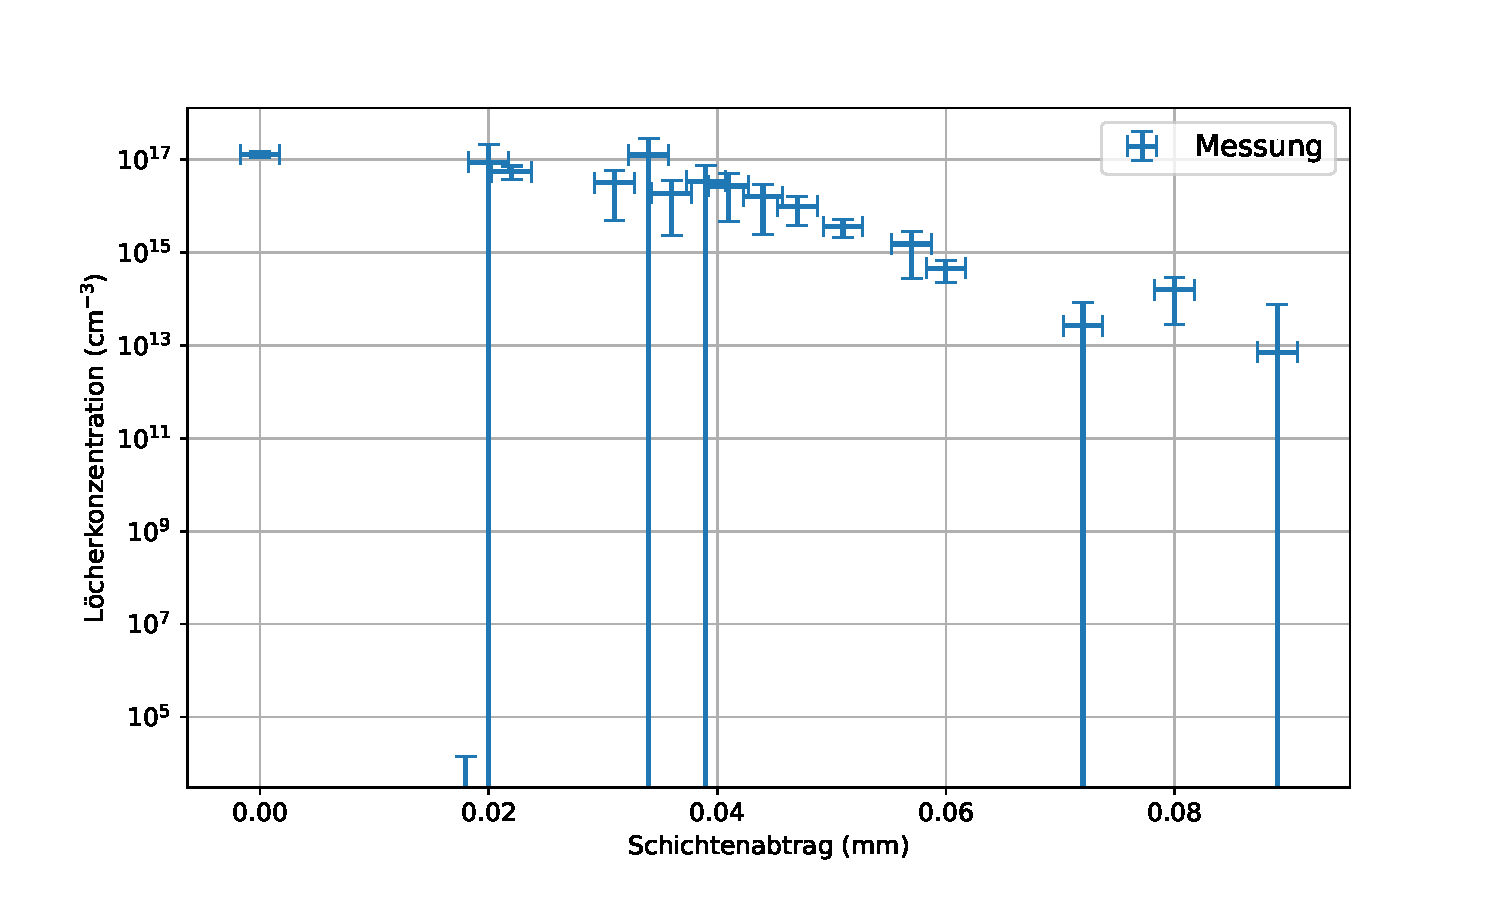
\includegraphics[width=\linewidth]{img/polier_konz.pdf}
			\caption{
			Löcherkonzentration in Abhängigkeit von dem Schichtenabtrag.
							}
			\label{fig_polier_konz}
	\end{figure}

	Der Mittelwert der letzten drei Löcherkonzentrationen beträgt \SI{0.9+-1.2e14}{cm^{-3}} und gibt die P-Grunddotierung an.
	Um die Konzentrationsverteilung der Ga-Atome zu erhalten muss die P-Grunddotierung von der Löcherkonzentration subtrahiert werden.
	Im Bereich von \SI{0}{\mu m} bis \SI{60}{\mu m} führt dies zu keiner merklichen Änderung der Löcherkonzentration, sodass in diesem Bereich in \cref{fig_polier_konz} die Konzentrationsverteilung der Ga-Atome entnommen werden kann.
	Nach \SI{65}{\mu m} ist die  Konzentration nahe Null.

	\subsubsection{Diskussion}
	%TODO diskus error von P-Grunddotierung
	%TODO Ausreißer bei 0.02 weil zu kleiner mess wert
	%TODO Ausreißer/Lock  bei 0.065 weil riesen sprung negativ => nicht aufgeführt
	%TODO Angabe zu intrinsisch bestätigen
	%TODO 70 mu m bestätigen
	In \cref{tb_dot_konz} sind die ermittelten Ladungsträgerkonzentrationen angegeben.
	Da hierfür keine Referenzwerte bekannt sind, kann kein Vergleich vorgenommen werden.
	Es kann aber festgestellt werden, dass in den dotierten Proben die eine Art der Ladungsträger um ein Vielfaches überwiegt und größer ist als im intrinsischen Halbleiter.
	Dass der spezifische Widerstand für dotierte Halbleiter um Größenordnungen geringer ist als für intrinsische Halbleiter ergibt sich aus den Beschreibungen im Theorieteil und kann anhand von \cref{tb_spez_wd} bestätigt werden.
	Außerdem kann die Gültigkeit der vorgenommenen Rechnungen aufgrund der Übereinstimmung mit den DIN-Tabellen gezeigt werden.

	Bei der schichtweisen Messung kann zunächst in \cref{fig_polier_wdst} festgestellt werden, dass der Widerstand mit zunehmender Messtiefe zunimmt und dann bei etwa \SI{65}{\micor \meter} auf ein konstantes Niveau fällt.
	Dieses Verhalten lässt sich vollständig aufgrund des Vorwissens über die Struktur der Probe erklären.
	Im Bereich nahe der Oberfläche überwiegt die Konzentration der Galliumatome gegenüber den Phosphor-Atomen und die Löcher sind Majoritätsladungsträger.
	Diese können sich frei bewegen und der Widerstand ist gering.
	Mit zunehmender Tiefe nimmt die Konzentration der Galliumatome ab, bis der Punkt erreicht ist, an dem die Konzentration der Galliumatome genauso groß wie die der Phosphoratome ist.
	An diesem Punkt kombinieren die meisten Löcher durch die Galliumdotierung mit Valenzelektronen der Phosphordotierung und die resultierende Gesamtladungsträgerkonzentration wird gering.
	Dementsprechend wurde hier ein Peak im Widerstand gemessen.
	Danach nimmt die Galliumkonzentration weiter ab (dieser Bereich konnte nicht gemessen werden), bis nur noch Phosphordotierung vorliegt.
	Hier steigt die Ladungsträgerkonzentration wieder und der Widerstand sinkt bis auf den Grenzwert durch die Phosphordotierung.

	\subsection{Solarzelle}

	Da keine eigenen Messungen zu den Solarzellen durchgeführt werden konnten, werden im folgenden alte Messdaten, die uns freundlicherweise von Finn Kutschmann ausgehändigt wurden, ausgewertet. %TODO fine?
	\subsubsection{Unsicherheiten}
	Für die erhaltenen Daten wurde immer eine Rechteckverteilung, ähnlich wie bei einer Digitalanzeige, angenommen.
	\subsubsection{Beobachtung und Datenanalyse}

	In \cref{fig_poly_unbeleuchtet_20} und \cref{fig_tandem_unbeleuchtet_20} sind die aufgenohmenen I-U-Kennlinien der polykristallinen Silizium Solarzelle und der Tandemzelle abgebildet.

	\begin{figure}[H]
			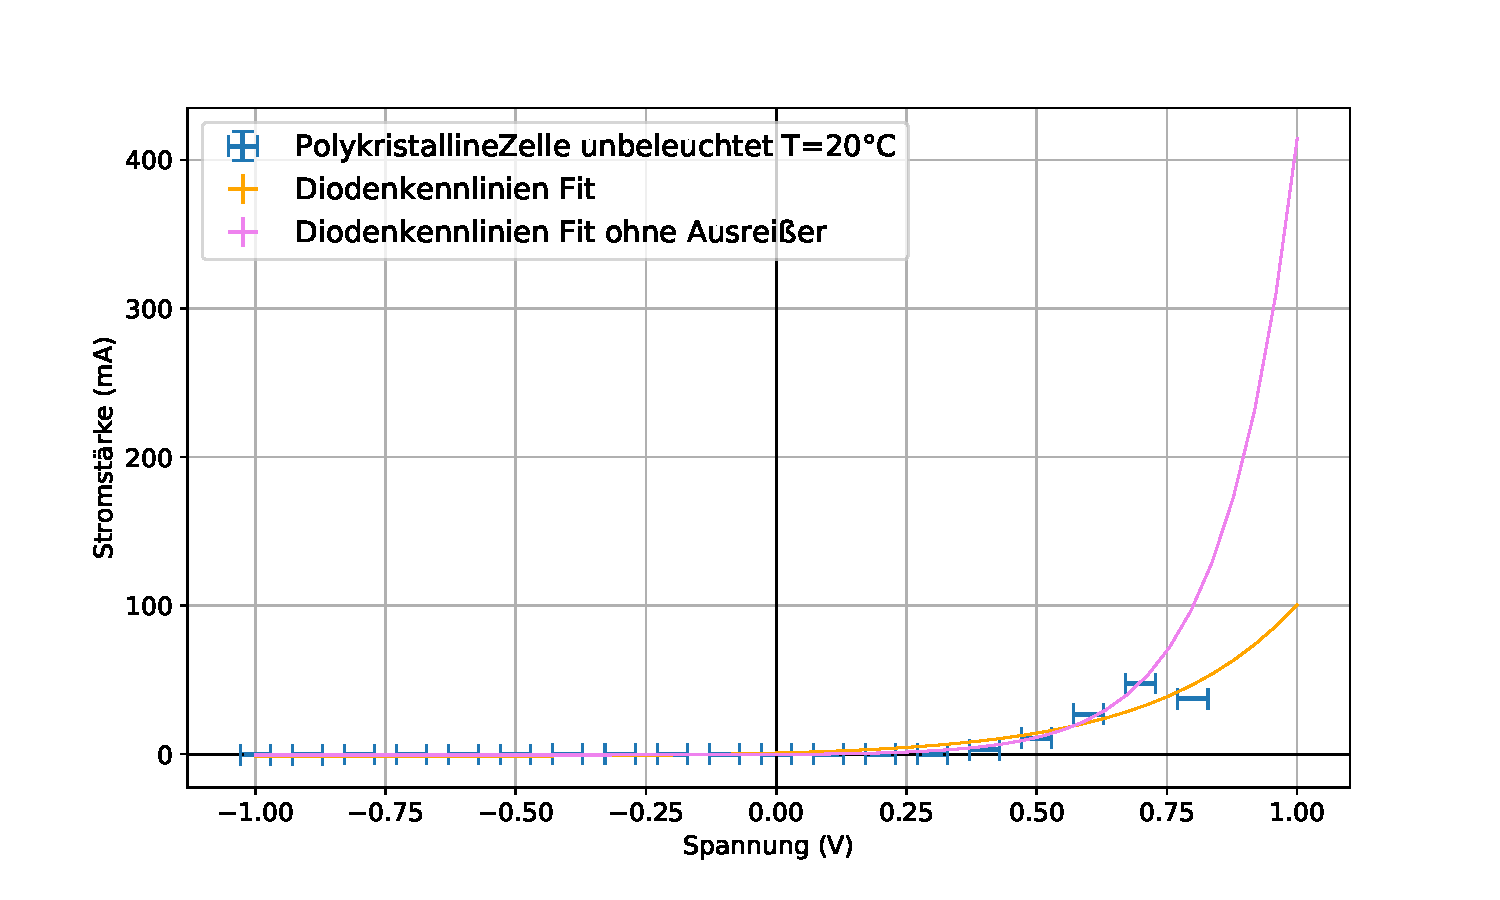
\includegraphics[width=.9\linewidth]{img/PolykristallineZelle_unbeleuchtet_20.pdf}
			\caption{
				I-U-Kennlinie einer polykristallinen Silizium Solarzelle bei Raumtemperatur ohne Beleuchtung.
				Der Diodenkennlinien-Fit erreicht deutlich geringere Abweichungen von den Messwerten unter Vernachlässigung des Messwerts bei $U=\SI{0.8}{V}$, weshalb im Bild beide Varianten dargestellt sind.
								}
			\label{fig_poly_unbeleuchtet_20}
	\end{figure}

	\begin{figure}[H]
			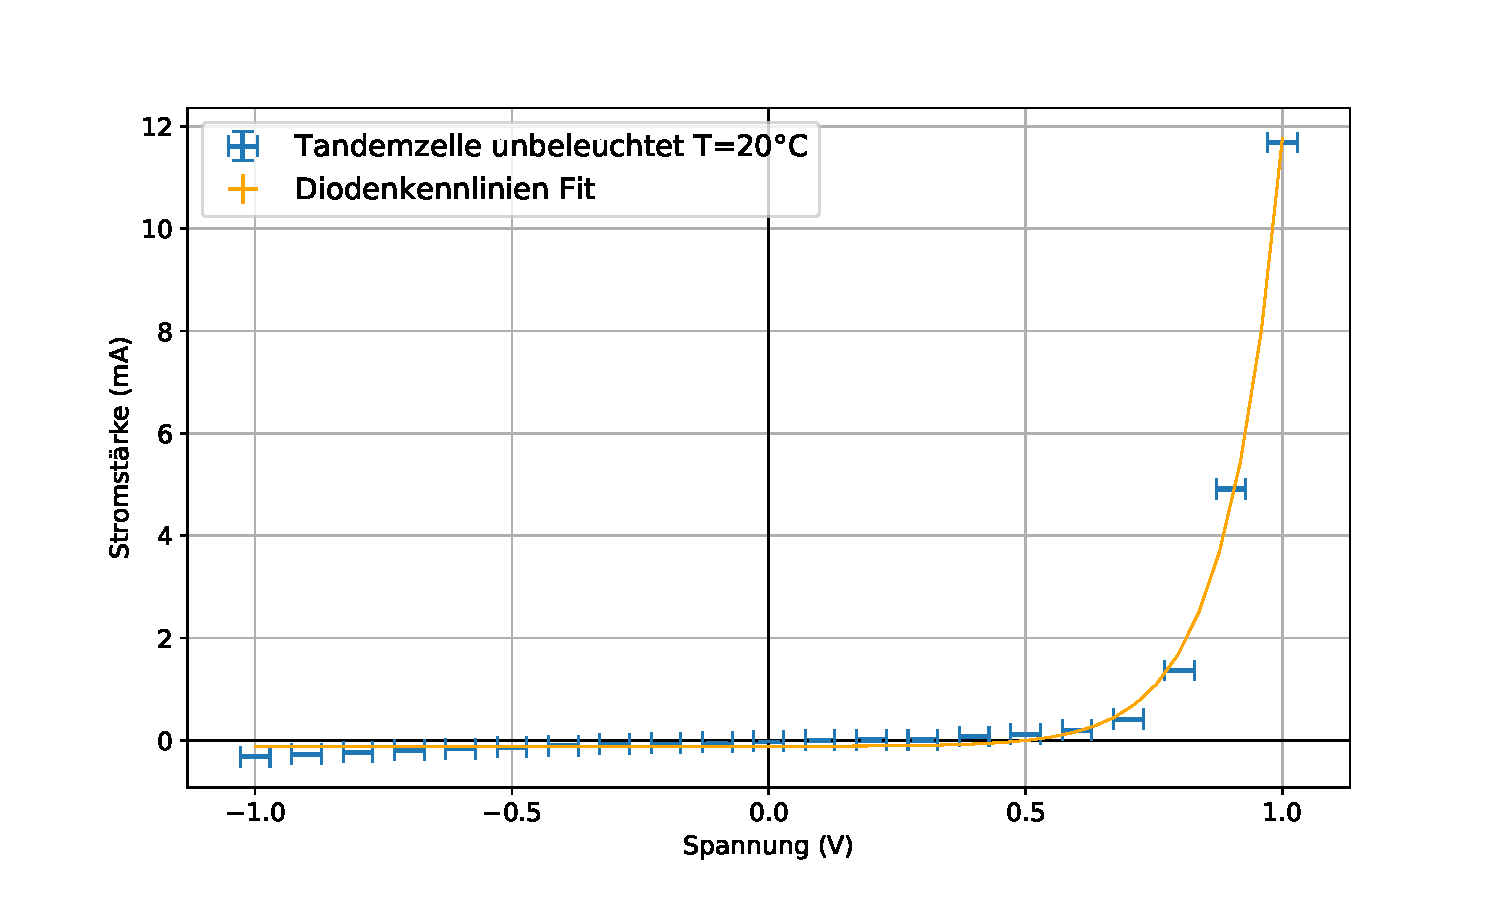
\includegraphics[width=.9\linewidth]{img/Tandemzelle_unbeleuchtet_20.pdf}
			\caption{
				I-U-Kennlinie einer Tandemzelle bei Raumtemperatur ohne Beleuchtung.
								}
			\label{fig_tandem_unbeleuchtet_20}
	\end{figure}

	Die Fitfunktion ist die ideale Diodenkennlinie unter Einstrahlung von Licht (vgl. \cref{eq_photostrom}).

	\cref{fig_tandem_beleuchtet_20} stellt exemplarisch die I-U-Kennlinie der Solarzellen dar, wenn sie mit Licht bestrahlt werden (weitere befinden sich im \nameref{s_anhang}).
	Das rote (grüne) Rechteck gibt die im 4. Quadranten durch $U_\text{MPP}$ und $I_\text{MPP}$ ($U_\text{oc}$ und $I_\text{sc}$) begrenzte Fläche an.
	Die rote Fläche entspricht der Maximalen Leistung $P_{max} = U_\text{MPP}I_\text{MPP}$.
	Der Füllfaktor $FF$ ergibt sich als das Verhältnis der Flächen, also
	\begin{equation}
		FF = \frac{U_\text{MPP}I_\text{MPP}}{U_\text{oc}I_\text{sc}}.
	\end{equation}
	Dabei konnten $U_\text{MPP}$, $I_\text{MPP}$ und $I_\text{sc}$ direkt aus den Messpunkten extrahiert werden.
	$U_\text{oc}$ musste mittels des Fits interpoliert werden.


	\begin{figure}[H]
			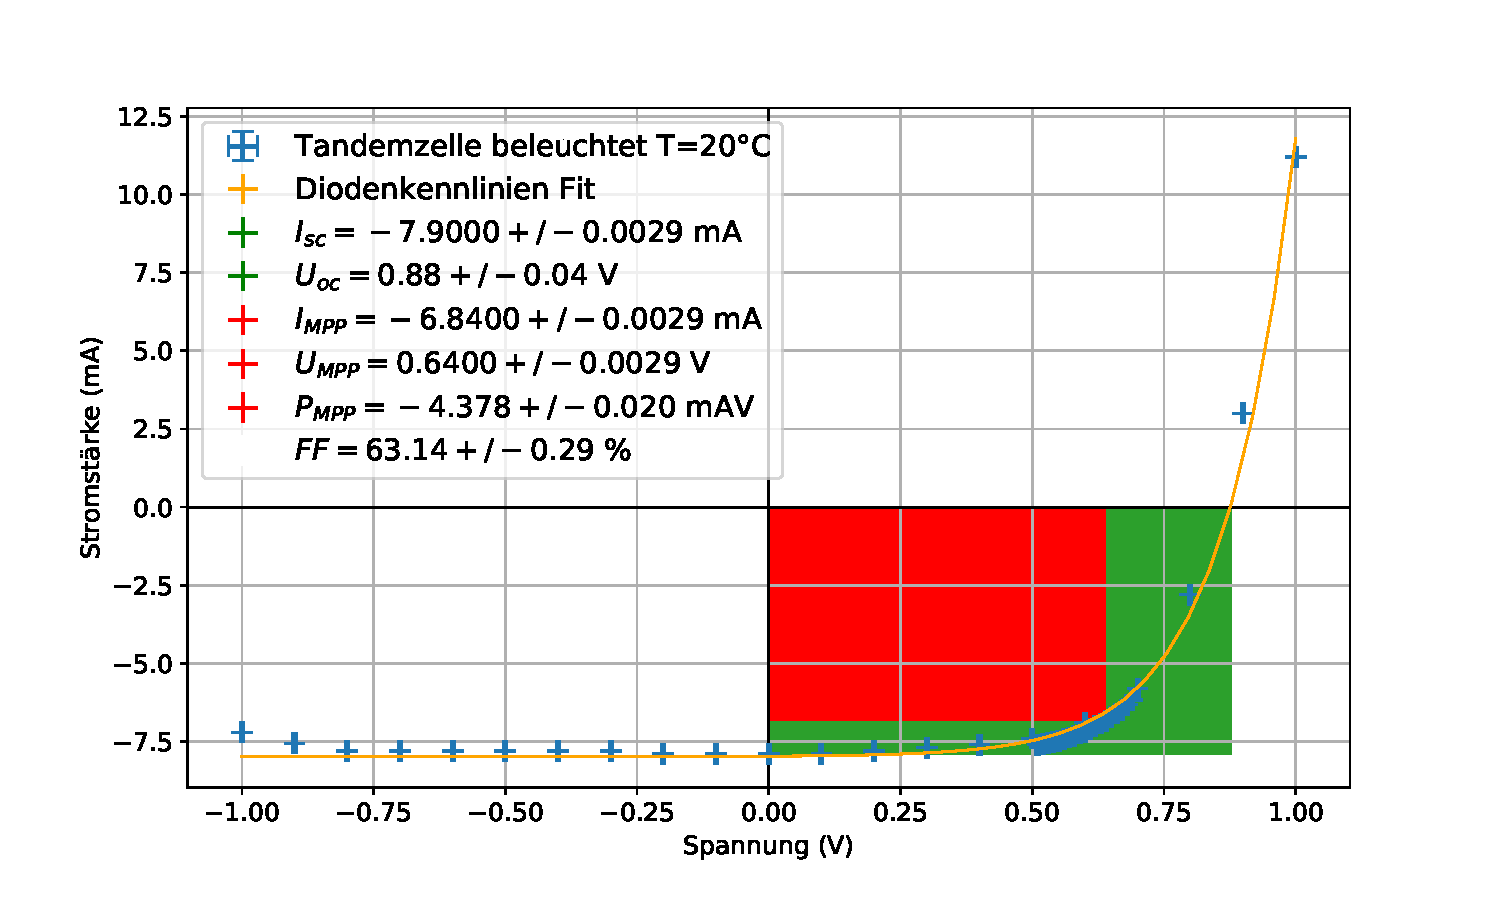
\includegraphics[width=.9\linewidth]{img/Tandemzelle_beleuchtet_20.pdf}
			\caption{
				I-U-Kennlinie einer Tandemzelle bei $T=\SI{20}{\celsius}$ unter Beleuchtung.
								}
			\label{fig_tandem_beleuchtet_20}
	\end{figure}
	In \cref{tb_solar_param_poly} und \cref{tb_solar_param_tandem} sind die wichtigsten Parameter der Solarzellen die unter Variation der Temperatur bestimmt wurden aufgeführt.

\begin{table}[H]
		\centering
		\begin{tabular}{c | c | c | c  }
			 &$T=\SI{20}{\celsius}$& $T=\SI{35}{\celsius}$& $T=\SI{50}{\celsius}$ \\ \hline
			 $I_\text{sc}$ in \si{mA}& \SI{151+-0.3}{}&\SI{149+-0.3}{}& \SI{147+-0.3}{} \\
			 $U_\text{oc}$ in \si{V}&\SI{0.63+-0.04}{}&\SI{0.61+-0.04}{}&\SI{0.61+-0.05}{} \\
			 $I_\text{MPP}$ in \si{mA}&\SI{108+-0.3}{}&\SI{99+-0.3}{}&\SI{96+-0.3}{} \\
			 $U_\text{MPP}$ in \si{V}&\SI{0.31+-0.003}{}&\SI{0.32+-0.003}{}&\SI{0.31+-0.003}{} \\
			 $P_\text{MPP}$ in \si{mW}&\SI{33.48+-0.32}{}&\SI{31.68+-0.3}{}&\SI{29.76+-0.3}{} \\
			 $FF$ in \si{\percent}&\SI{35.05+-2.5}{}&\SI{34.8+-2.5}{}&\SI{33+-2.7}{} \\
		\end{tabular}
		\caption{
		Beträge der wichtigen Parameter der polykristalline Zelle bei verschieden Temperaturen.
		}
		\label{tb_solar_param_poly}
\end{table}

\begin{table}[H]
		\centering
		\begin{tabular}{c | c | c | c  }
			 &$T=\SI{20}{\celsius}$& $T=\SI{50}{\celsius}$& AM-Filter $T=\SI{20}{\celsius}$ \\ \hline
			 $I_\text{sc}$ in \si{mA}& \SI{7.9+-0.003}{}&\SI{5.42+-0.003}{}& \SI{0.94+-0.003}{} \\
			 $U_\text{oc}$ in \si{V}&\SI{0.88+-0.04}{}&\SI{0.776+-0.032}{}&\SI{0.705+-0.024}{} \\
			 $I_\text{MPP}$ in \si{mA}&\SI{6.84+-0.03}{}&\SI{4.24+-0.003}{}&\SI{0.700+-0.003}{} \\
			 $U_\text{MPP}$ in \si{V}&\SI{0.64+-0.003}{}&\SI{0.60+-0.003}{}&\SI{0.54+-0.003}{} \\
			 $P_\text{MPP}$ in \si{mW}&\SI{4.378+-0.022}{}&\SI{2.544+-0.012}{}&\SI{0.378+-0.003}{} \\
			 $FF$ in \si{\percent}&\SI{63.3+-2.8}{}&\SI{60.5+-2.5}{}&\SI{57+-2.0}{} \\
		\end{tabular}
		\caption{
		Beträge der wichtigen Parameter der Tandemzelle bei verschiedenen Temperaturen und Lichtspektren.
		}
		\label{tb_solar_param_tandem}
\end{table}
	\subsubsection{Diskussion}
	Da die Messungen nicht selbst durchgeführt wurden, kann nicht geklärt werden, worauf der \enquote{Ausreißer} in den Messwerten in \cref{fig_poly_unbeleuchtet_20} zurückzuführen ist.
	Wie anhand der Fits in \cref{fig_poly_unbeleuchtet_20} und \cref{fig_tandem_unbeleuchtet_20} zu erkennen ist, verhalten sich die Solarzellen insgesamt aber beide erwartungsgemäß wie Dioden.

	Da in \cref{eq_photostrom} $I_\text{ph}$ der vertikalen Verschiebung an der Ordinate entspricht, wird erwartet, dass dieser nahe Null ist, wenn die Solarzelle nicht beleuchtet wird.
	Dies ist in \cref{fig_poly_unbeleuchtet_20} und \cref{fig_tandem_unbeleuchtet_20} innerhalb der Messunsicherheiten erfüllt.
	Letztere können auf Hintergrundlicht oder thermischen Schwankungen beruhen.

	In \cref{tb_solar_param_poly} und \cref{tb_solar_param_tandem} ist deutlich zu erkennen, dass bei beiden Solarzellen der Füllfaktor und die Spannung am MPP mit der Temperatur abnimmt.
	Dies liegt daran, dass mit steigender Temperatur die Größe der Bandlücke sinkt, sodass die angeregten Elektronen durch graduelle Abstrahlung energetisch tiefer sinken können und somit mehr Energie verlieren, die nicht in elektrische Leistung umgesetzt werden kann.
	Der AM-Filter reduziert die Spannung am MPP massiv, was daran liegt, dass weniger Lichtleistung für die Zelle zur Verfügung steht, da einige Wellenlängen herausgefiltert wurden.

	Es wäre zu erwarten, dass der Wirkungsgrad der Tandemzelle höher ist, als der der polykristallinen Siliziumzelle, da diese aus mehreren pn-Übergängen übereinander besteht, welche die Absorption eines breiteren Lichtspektrums erlauben.
	Da die Leistung des einfallenden Lichts nicht bekannt ist, kann der Wirkungsgrad jedoch nicht bestimmt werden.
	Die Füllfaktoren wären nur vergleichbar, wenn eine gleich große Fläche der Zelle mit der gleichen Lampe beschienen werden würde.
	Ersteres war jedoch nicht der Fall.

	% Allgemeine Beobachtungen
	% Einflüsse von veränderten Parametern auf Messung
	% Berechung nach Aufgabenstellung

	% Bezug/Nutzen oder sonst was
	% auch hier die Hypothese wiederholen
	% keine Messwerte hier, nach manchen Menschen, zumindest "direkt" erstellte Diagramme net hier, auch wenn Lesbarkeit-bla

	\section{Schlussfolgerung}
	% Rückgriff auf Hypothese und drittes Nennen dieser
	Insgesamt gesehen konnten die geplanten Messungen durchgeführt werden und die Eigenschaften der untersuchten Halbleiter und Solarzellen erfolgreich untersucht werden.
	So konnten bei den Halbleitern die Ladungsträgerkonzentrationen bestimmt werden und gezeigt werden, dass intrinsische Halbleiter den elektrischen Strom um Größenordnungen schlechter leiten als dotierte Halbleiter.
	es wurde ein Schichtprofil der Ladungsträgerkonzentration in einem Halbleiter mit tiefenabhängiger Dotierung erstellt.
	Die Güte dieses Profils litt jedoch unter der ungenauen Methode des Abpolierens des Halbleiters.
	Die Untersuchung einer polykristallinen Siliziumzelle und einer Tandemzelle erlaubte die Bestimmung des Maximum Power Points und des Füllfaktors.
	Der Zusammenhang dieser beiden Eigenschaften mit der Temperatur konnte ebenfalls untersucht werden.
	Ein Vergleich der beiden Zellen war jedoch aufgrund mangelnder gleicher Versuchsbedingungen nicht möglich.
	Wenn die Leistung des einfallenden Lichts bekannt gewesen wäre, wäre es möglich gewesen, den Wirkungsgrad der Solarzellen zu bestimmen.

	% Quellen zitieren, Websiten mit Zugriffsdatum
	% Verweise auf das Laborbuch (sind erlaubt)
	% Tabelle + Bilder mit Beschriftung
	\printbibliography

	%TODO Anhang notwendig?
	\section{Anhang} \label{s_anhang}
	\subsection{Solarzelle}
	\begin{figure}[H]
			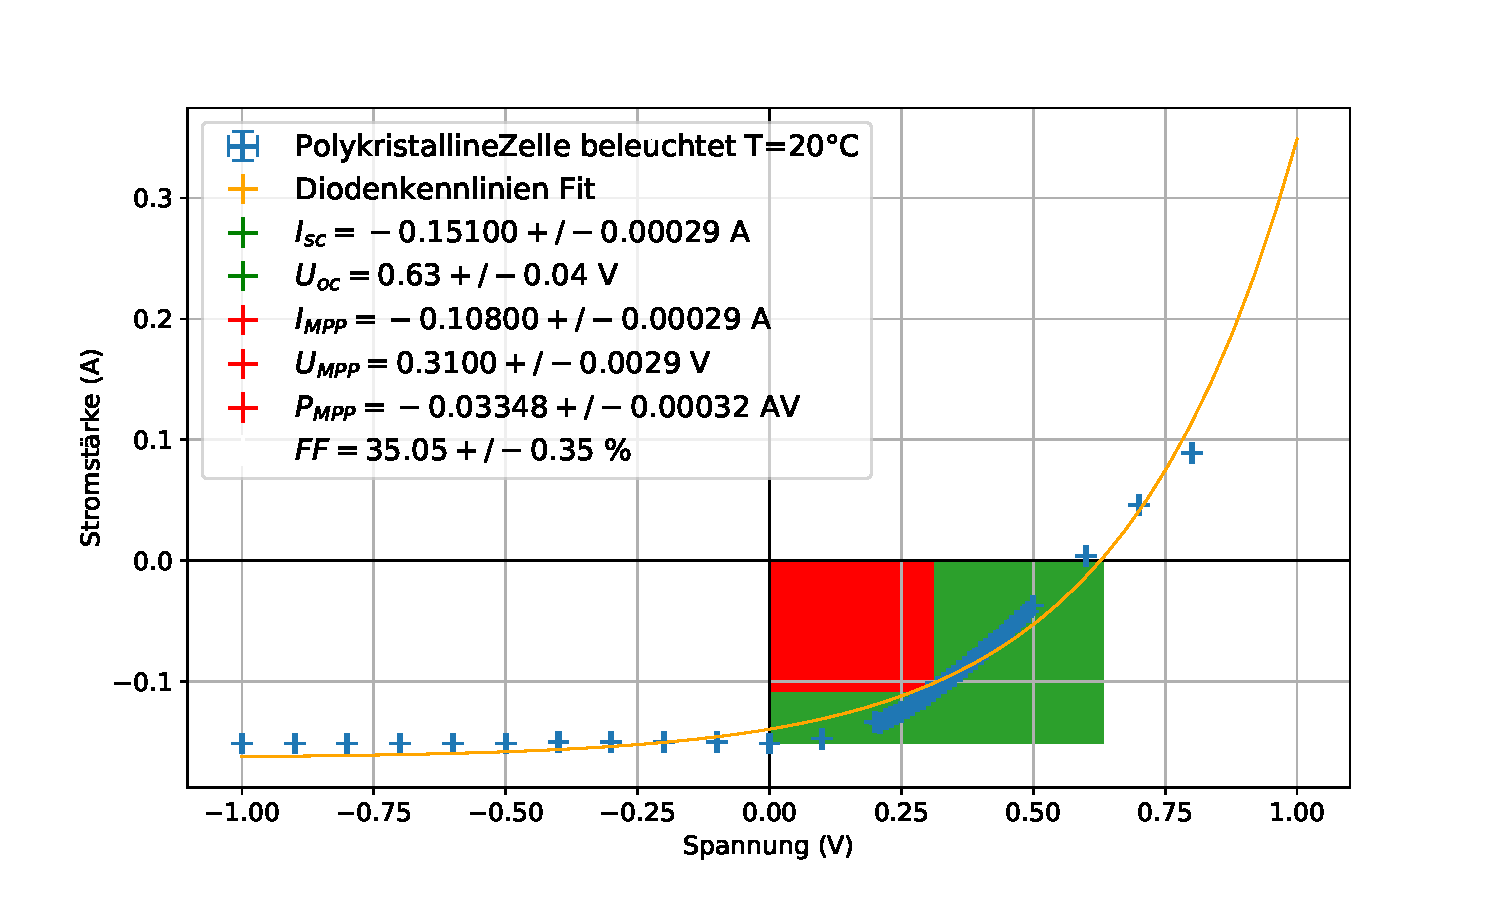
\includegraphics[width=.9\linewidth]{img/PolykristallineZelle_beleuchtet_20.pdf}
			\caption{
				I-U-Kennlinie einer polykristallinen Silizium Solarzelle bei Raumtemperatur unter Beleuchtung.
								}
			\label{fig_poly_beleuchtet_20}
	\end{figure}
	\begin{figure}[H]
			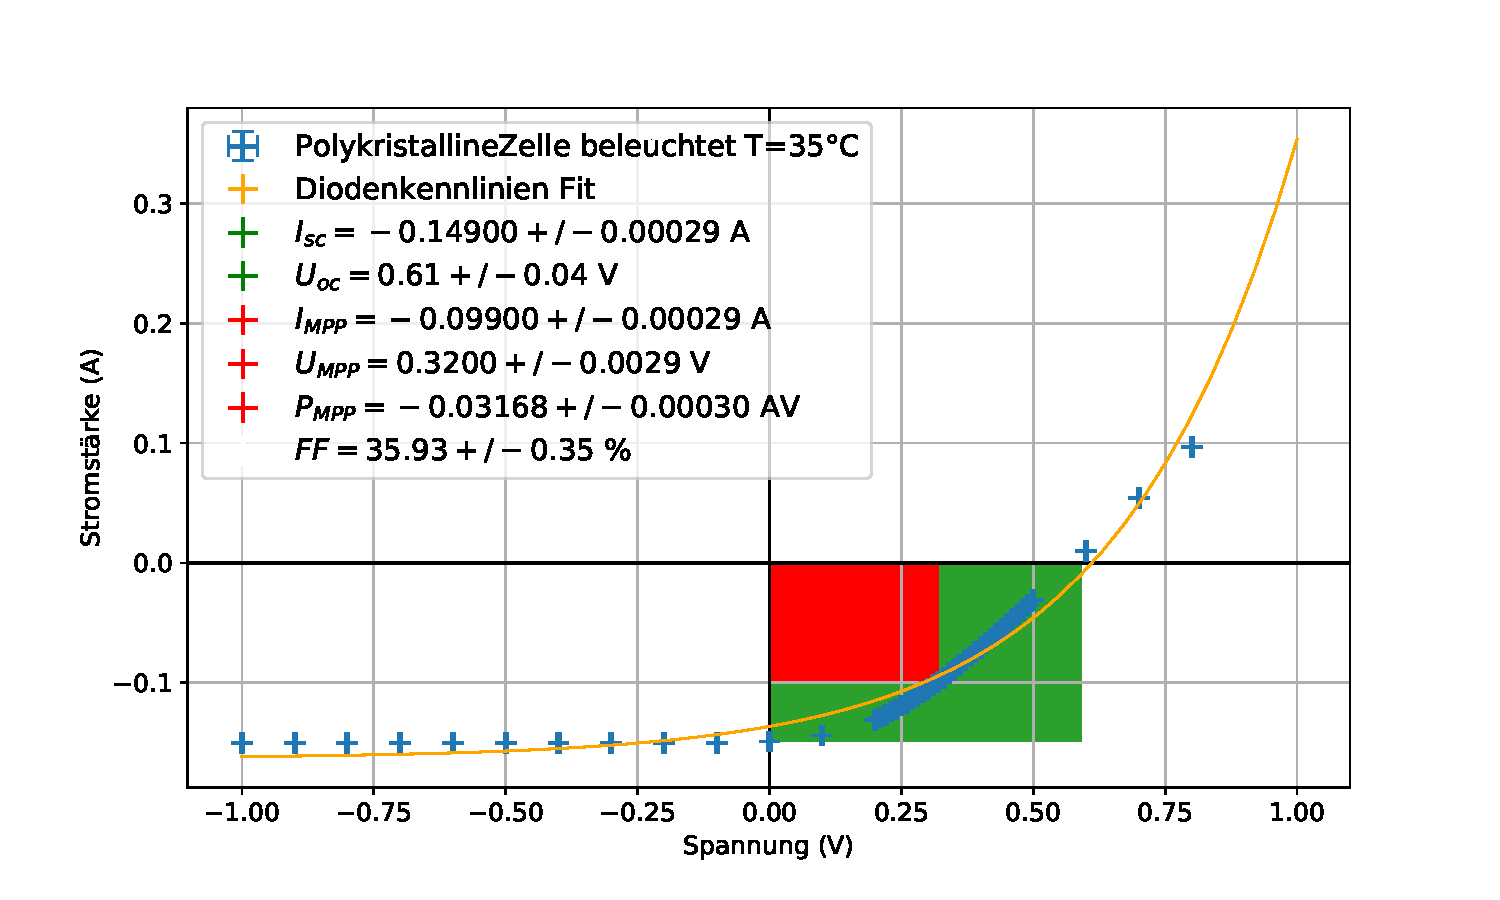
\includegraphics[width=.9\linewidth]{img/PolykristallineZelle_beleuchtet_35.pdf}
			\caption{
				I-U-Kennlinie einer polykristallinen Silizium Solarzelle bei $T=\SI{35}{\celsius}$ unter Beleuchtung.
								}
			\label{fig_poly_beleuchtet_35}
	\end{figure}

	\begin{figure}[H]
			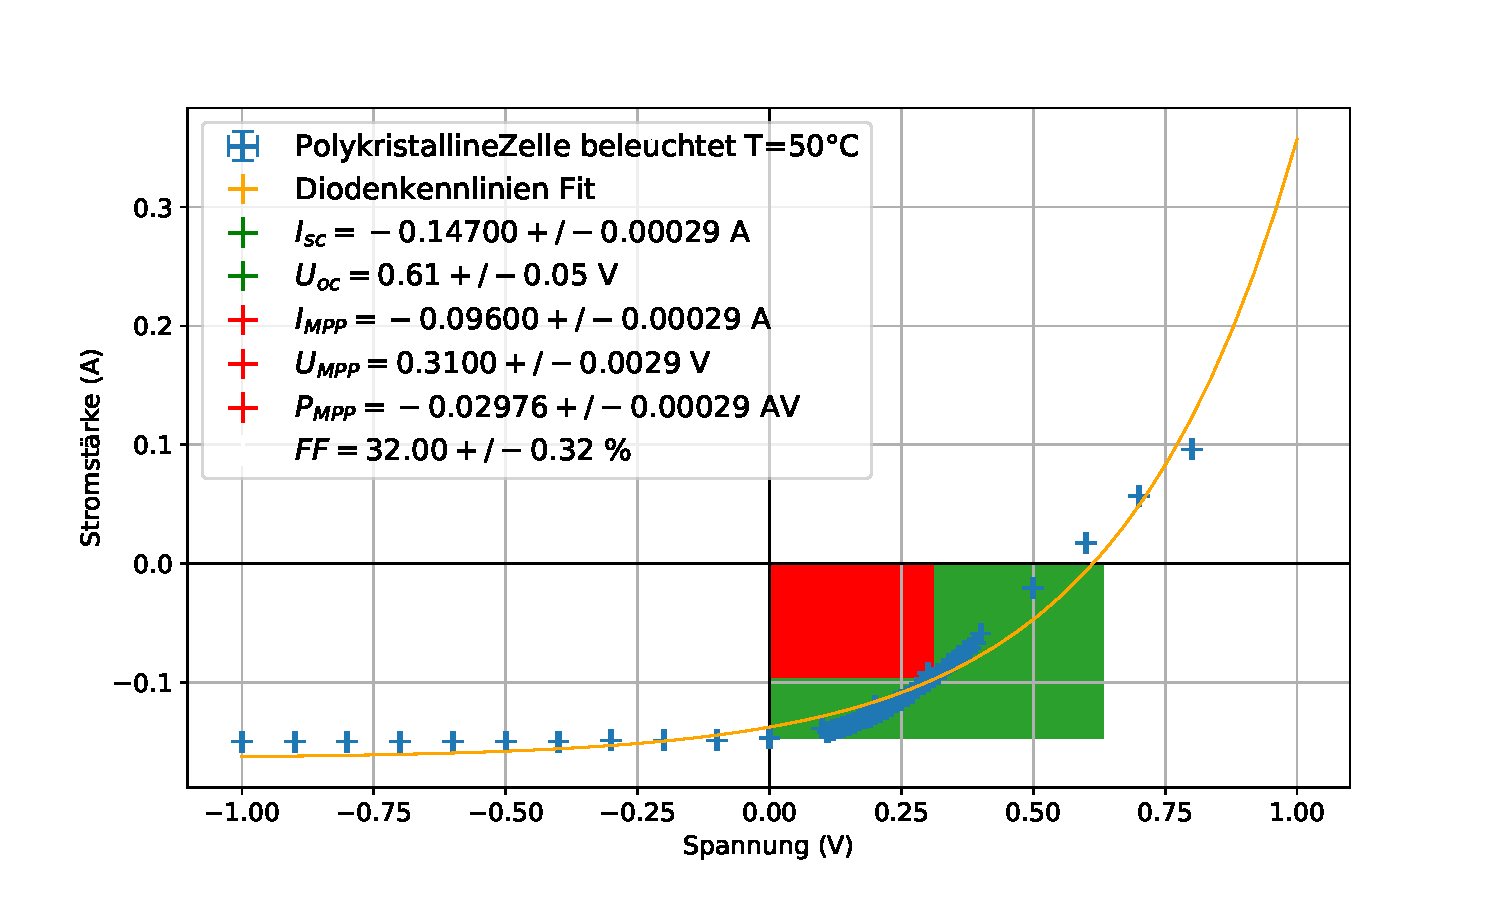
\includegraphics[width=.9\linewidth]{img/PolykristallineZelle_beleuchtet_50.pdf}
			\caption{
				I-U-Kennlinie einer polykristallinen Silizium Solarzelle bei $T=\SI{50}{\celsius}$ unter Beleuchtung.
								}
			\label{fig_poly_beleuchtet_50}
	\end{figure}


	\begin{figure}[H]
			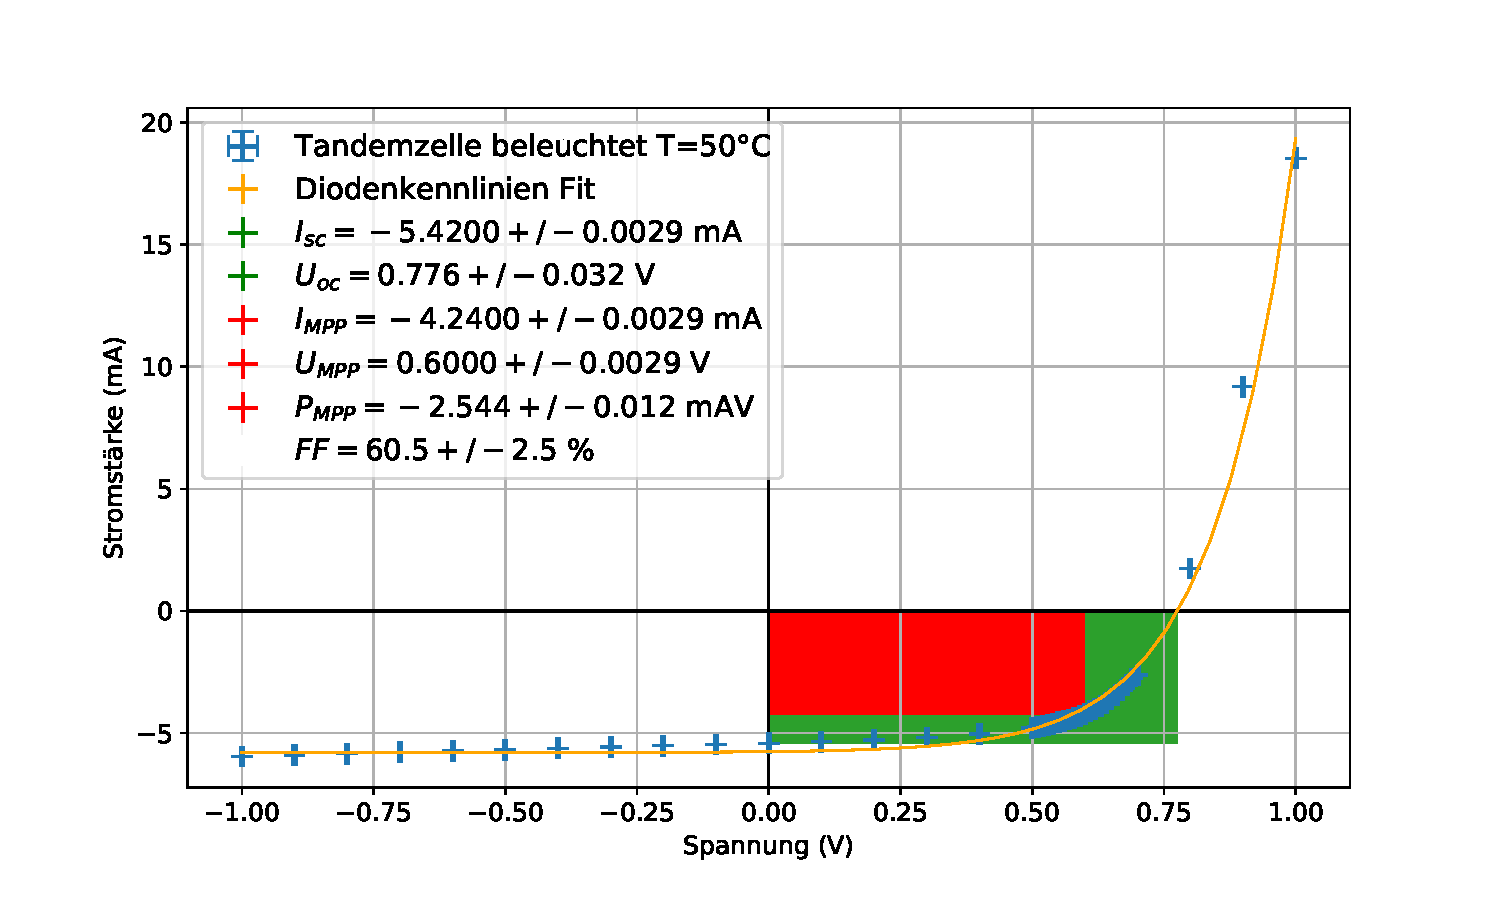
\includegraphics[width=.9\linewidth]{img/Tandemzelle_beleuchtet_50.pdf}
			\caption{
				I-U-Kennlinie einer Tandemzelle bei $T=\SI{50}{\celsius}$ unter Beleuchtung.
								}
			\label{fig_tandem_beleuchtet_50}
	\end{figure}

	\begin{figure}[H]
			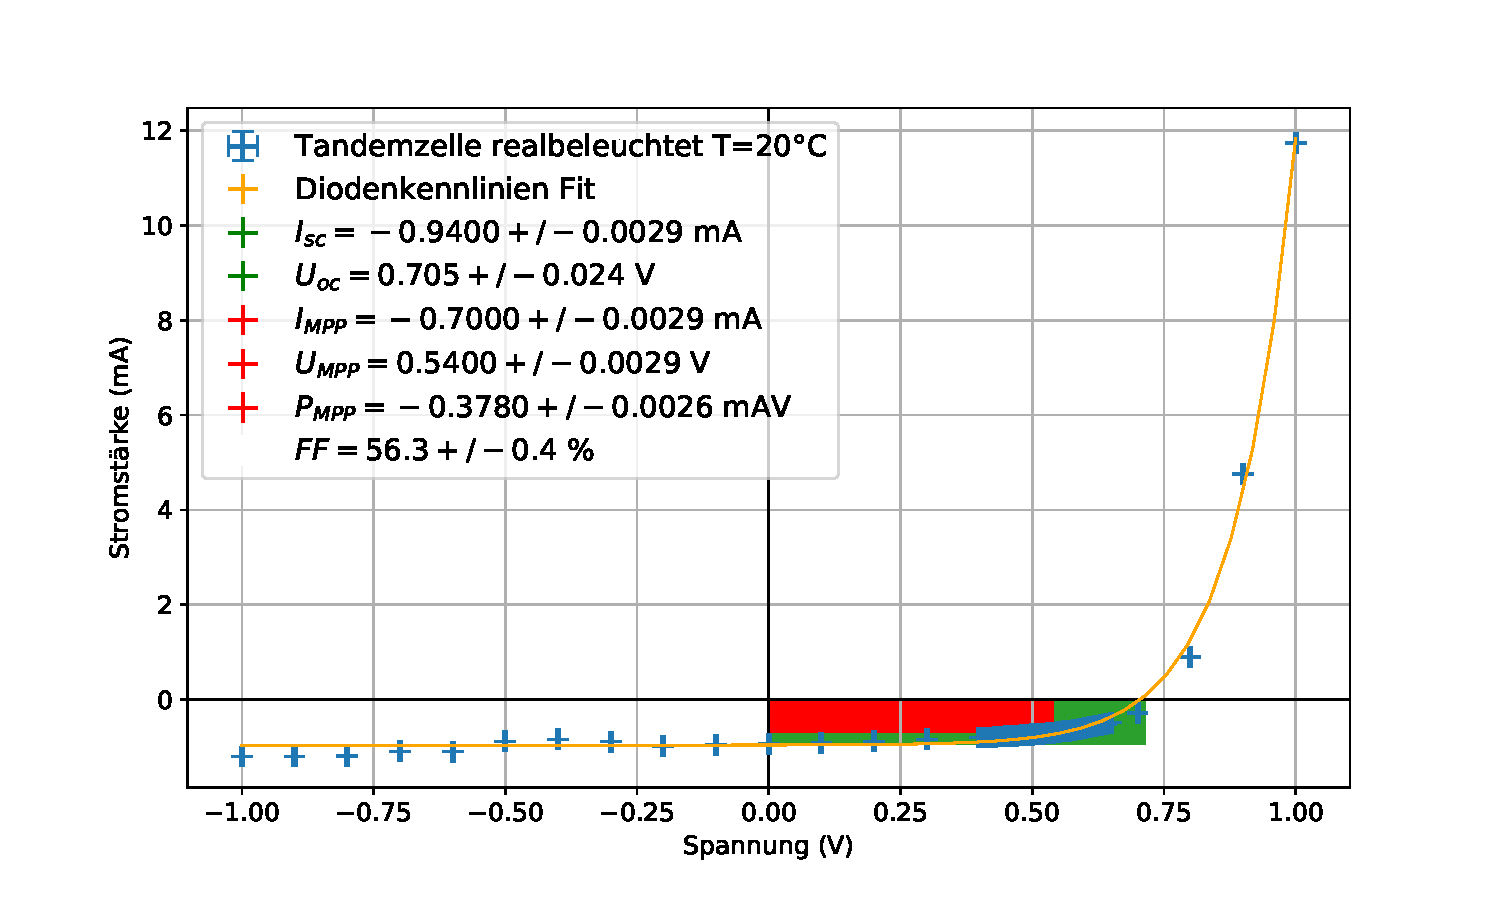
\includegraphics[width=.9\linewidth]{img/Tandemzelle_realbeleuchtet_20.pdf}
			\caption{
				I-U-Kennlinie einer Tandemzelle bei Raumtemperatur unter Beleuchtung durch einen AM-Filter.
			}
			\label{fig_tandem_realbeleuchtet_20}
	\end{figure}
\end{document}
